\documentclass[12pt]{article}

\usepackage{lineno}

%% User packages
\usepackage{amsmath}
\usepackage{amssymb}
\usepackage{amsfonts}
\usepackage{graphicx}
\usepackage{tikz}
\usepackage{pgfplots}
\usepackage{amsthm}
\usepackage{cancel}
\usepackage{caption}
\usepackage{natbib}
\usepackage[margin=1in]{geometry}

%% User definitions
\newtheorem{theorem}{Theorem}
\newtheorem{corollary}{Corollary}
\newtheorem{proposition}{Proposition}
\newtheorem{example}{Example}
\allowbreak

\pgfplotsset{every axis/.append style={
                axis x line=middle,
                axis y line=middle,
                axis line style={->},
            }}


\bibliographystyle{abbrvnat}

\title{Carryover of a saddle-node bifurcation after transformation of a parameter into a variable}
\author{Carlos Contreras, Gustavo Carrero, Gerda de Vries}
% \address{University of Alberta}




\begin{document}

\maketitle


\begin{abstract}
To do.

Saddle-Node Bifurcation, Carryover, Bifurcations
\end{abstract}
 

\linenumbers


Consider the dimensionless model for the activation of gen $x$ by biochemical substance $s$
\begin{equation}
    \dot x = s - rx + \frac{x^{2}}{1+x^{2}},
    \label{equ:Example:GenActivation:1D}
\end{equation}
where $r>0$ is the degradation rate and $s\geq0$ \citep{Strogatz1994, Lewis1977}. This model is characterized by an irreversible switch-like activation (critical transition) of gen when $s$ increases from zero above a threshold. Suppose that we incorporate the dynamics of $r$ into the system, can we preserve the critical transition characteristic? and if so, can we determine conditions for that? The critical transition is determined by a critical saddle-node bifurcation in which the stable equilibrium for low gen activity collides with an unstable equilibrium, leading trajectories towards the remaining stable equilibria for high gen activity. If $r$ is transformed into a variable, we would expect the same critical saddle-node bifurcation to occur but in a higher dimension. In that case, we say that we extend the smaller system and that we carryover the bifurcation to the extended system. In this paper, we provide conditions for the carryover property and apply our results to two model in mathematical biology.

% Saddle-node bifurcations are very common in biology, medicine and ecology [references, eg. Li et al. 2019], explaining hysteresis and critical transitions. 


In the general case, we are interested in the conditions such that a saddle-node bifurcation for the system
\begin{equation}
    \dot z = f(z;\mu_{1},\mu_{2}),
    \label{equ:OriginalSystem}
\end{equation}
where $z\in\mathbb{R}^{n}$ and $\mu_{1},\mu_{2}\in\mathbb{R}$, manifests itself after we extend the system by transforming one of the parameters, for example, $\mu_{1}$, into a variable. This defines the extended system
\begin{equation}
    \left. \begin{aligned}
    \dot z &= f(z,\mu_{1}; \mu_{2}), \\
    \dot \mu_{1} &= g(\mu_{1}; \mu_{2}),
    \end{aligned} \right.
    \label{equ:ExtendedSystem}
\end{equation}
where a saddle-node bifurcation occurs and $g(\mu_{1}; \mu_{2})$ is the vector field of the new variable $\mu_{1}$. We call this saddle-node the carryover of a saddle-node bifurcation in the original system \eqref{equ:OriginalSystem} to the extended system \eqref{equ:ExtendedSystem}. Note that the function $g$ does not depend on $z$. The case where $g$ depends on $z$ is beyond the scope of this chapter, but we briefly discuss this case in Section~\ref{sec:Discussion}.

Saddle-node bifurcations in $\mathbb{R}^{n}$ are characterized by three conditions: singularity, nondegeneracy, and transversality conditions. They guarantee the creation (or destruction) of two equilibria as one parameter crosses the bifurcation value. This is summarized in the following results taken from \citet[Ch. 8]{Meiss2007}.

\begin{theorem}[saddle node]
    \label{the:SaddleNodeBifurcationND}
    Let $f\in C^2(\mathbb{R}^n\times \mathbb{R}^k,\mathbb{R}^n)$, and suppose that $f(z;\mu$) satisfies
    \begin{equation}
        f(0;0)=0, \quad \mathrm{spec}(D_z f(0;0))=\{ 0, \lambda_2, \lambda_3, \ldots, \lambda_n : \lambda_k \neq 0, k\neq 1 \}.
        \label{equ:SaddleNodeBifurcationND:Singularity}
    \end{equation}
    Choose coordinates so that $D_zf(0;0)$ is diagonal in the zero eigenvalue and set $z=(x,y)$ where $x\in \mathbb{R}^1$ corresponds to the zero eigenvalue and $y\in \mathbb{R}^{n-1}$ are the remaining coordinates. Then 
    \begin{equation}
        \begin{split}
            \dot x &= f_1(x,y;\mu), \\
            \dot y &= My + f_2(x,y;\mu),
        \end{split}
        \label{equ:SaddleNodeBifurcationND:System}
    \end{equation}
    where $f_{1}(0,0;0)=0$, $f_{2}(0,0;0)=0$, $D_z f_{1}(0,0;0)=0$, $D_z f_{2}(0,0;0)=0$, and $M$ is an invertible matrix. Suppose that 
    \begin{equation}
        D_{xx}f_1(0,0;0)=c\neq 0.
        \label{equ:SaddleNodeBifurcationND:Nondegeneracy}
    \end{equation}
    Then there exists an interval $I(\mu)$ containing $0$, functions $y=\eta(x;\mu)$ and extremal value $m(\mu)=\mathop{\mathrm{Ext}}_{x\in I(\mu)}[f_1(x;\eta(\mu);\mu)]$, and a neighborhood of $\mu=0$ such that if $m(\mu)c>0$ there are no equilibria and if $m(\mu)c<0$ there are two. Suppose that $M$ has a $u$-dimensional unstable space and an $(n-u-1)$-dimensional stable space. Then, when there are two equilibria, one has a $u$-dimensional unstable manifold and an $(n-u)$-dimensional stable manifold and the other has a $(u+1)$-dimensional unstable manifold and an $(n-u-1)$-dimensional stable manifold.
\end{theorem}

Equations \eqref{equ:SaddleNodeBifurcationND:Singularity} and \eqref{equ:SaddleNodeBifurcationND:Nondegeneracy} are the singularity and nondegeneracy conditions, respectively. They are necessary conditions for the function $f_{1}$ to be zero up to the zero- and first-order approximations about the bifurcation point, but nonzero in the second-order approximation. The function $y=\eta(x;\mu)$ allows us to reduce the dynamics in a neighborhood of the bifurcation point to one-dimension, i.e.,
\begin{equation*}
    \dot x = f_{1}(x,\eta(x;\mu);\mu).
\end{equation*}
The extremal value function $m(\mu)$ determines a single condition on the parameters, $m(\mu)=0$, along which two equilibria are created (or destroyed). Having one condition on the parameters means that the bifurcation that takes place has codimension-one. In order to be a saddle-node bifurcation, the equilibria need to be created as a some combination of the parameters crosses the bifurcation point. This can be guaranteed with a simple condition.

\begin{corollary}
    \label{the:SaddleNodeBifurcationNDCorollary}
    If $\mu_1$ is a single parameter such that 
    \begin{equation}
        D_{\mu_1}f_1(0,0;0)\neq 0,
        \label{equ:SaddleNodeBifurcationND:Transversality}
    \end{equation}
    then a saddle-node bifurcation takes place when $\mu_1$ crosses zero.
\end{corollary}

Equation \eqref{equ:SaddleNodeBifurcationND:Transversality} is the transversality condition that guarantees that $m(\mu)=0$ is crossed transversally as $\mu_{1}$ crosses zero. Note that $\mu_{1}$ is an arbitrary parameter, and that the transversality condition can hold for several parameters at the same time. We only consider saddle-node bifurcations that take place as a single parameter crosses the bifurcation point.

In the context of this chapter, we only consider two parameters for the sake of simplicity, i.e., $\mu=(\mu_{1},\mu_{2})\in\mathbb{R}^{2}$. We show that as long as a saddle-node bifurcation takes place in system \eqref{equ:OriginalSystem} for at least one of the parameters, the extended system \eqref{equ:ExtendedSystem} also has a saddle-node bifurcation for the other parameter (the extended variable does not have to be a bifurcation parameter in the original system) under some singularity and transversality conditions.

The Implicit Function Theorem is an essential tool in this chapter and in the study of saddle-node bifurcations in general. For example, the function $y=\eta(x;\mu)$ in Theorem~\ref{the:SaddleNodeBifurcationND} is consequence of this theorem. The following form of the Implicit Function Theorem is taken from \citet[Ch. 8]{Meiss2007}.
\begin{theorem}[implicit function]
    \label{the:ImplicitFunction}
    Let $U$ be an open set in $\mathbb{R}^{n}\times\mathbb{R}^{k}$ and $F\in C^{r}(U,\mathbb{R}^{n})$ with $r\geq 1$. Suppose there is a point $(x_{0},\mu_{0})\in U$ such that $F(x_{0};\mu_{0})=c$ and $D_{x}F(x_{0};\mu_{0})$ is a nonsingular matrix. Then there are open sets $V\subset \mathbb{R}^{n}$ and $W\subset \mathbb{R}^{k}$ and a unique $C^{r}$ function $\xi(\mu):W\mapsto V$ for which $x_{0}=\xi(\mu_{0})$ and $F(\xi(\mu);\mu)=c$.
\end{theorem}

This chapter is structured as follows. In Section \ref{sec:1DCase}, we look at the case where system \eqref{equ:OriginalSystem} is one dimensional, in which case we replace $z\in\mathbb{R}^{n}$ with $x\in\mathbb{R}^{1}$. We find conditions such that the two-dimensional extended system \eqref{equ:ExtendedSystem} has a saddle-node bifurcation. Moreover, we provide a graphical way to easily verify such conditions: the nullcline of the new equation ($g=0$ in the extended system \eqref{equ:ExtendedSystem}) has to intersect transversally the two-parameter bifurcation curve of the original system \eqref{equ:OriginalSystem}. Then, we apply our results to a few illustrative examples. In Section~\ref{sec:NDCase}, we expand our results to the $n$-dimensional case and apply our results to one illustrative example. Finally, in Section~\ref{sec:Discussion}, we discuss our results and further research.


\section{One-dimensional case}
\label{sec:1DCase}


In this section, we focus on the case where the variable $z$ in the system \eqref{equ:OriginalSystem} is one-dimensional, i.e., the system
\begin{equation}
    \dot x = f(x;\mu_{1},\mu_{2}),
    \label{equ:1DCase:OriginalSystem}
\end{equation}
where $x\in\mathbb{R}$, $\mu_{1},\mu_{2}\in\mathbb{R}$, and $f$ is a sufficiently smooth function on $(x,\mu_{1},\mu_{2})$. This system is extended by transforming one of the parameters, for example, $\mu_{1}$, into a variable to define the extended system
\begin{equation}
    \left. \begin{aligned}
    \dot x &= f(x,\mu_{1}; \mu_{2}), \\
    \dot \mu_{1} &= g(\mu_{1}; \mu_{2}),
    \end{aligned}\right.
    \label{equ:1DCase:ExtendedSystem}
\end{equation}
where $g(\mu_{1}; \mu_{2})$ is the sufficiently smooth vector field of the new variable $\mu_{1}$. We want to find conditions for the carryover of a saddle-node bifurcation in the original \eqref{equ:1DCase:OriginalSystem} to the extended system \eqref{equ:1DCase:ExtendedSystem}.


Suppose, without loss of generality, that the saddle-node bifurcation for \eqref{equ:1DCase:OriginalSystem} occurs at the origin as one parameter, $\mu_{1}$, crosses zero. That is, $f$ at $(x,\mu_{1}, \mu_{2})=(0,0,0)$ satisfies the singularity conditions
\begin{equation}
    \left\{ \begin{aligned}
    &f(x;\mu_{1},\mu_{2})=0, \\
    &D_{x}f(x;\mu_{1,\mu_{2}})=0,
    \end{aligned}\right.
    \label{equ:1DCase:SingularitySystem}
\end{equation}
and the nondegeneracy and transversality conditions
\begin{equation}
    \left\{ \begin{aligned}
    &D_{xx}f(x;\mu_{1},\mu_{2})\neq 0, \\
    &D_{\mu_{1}}f(x;\mu_{1},\mu_{2})\neq 0.
    \end{aligned}\right.
    \label{equ:1DCase:NondegeneracyAndTransversalitySystem}
\end{equation}

Note that system \eqref{equ:1DCase:SingularitySystem} has two equations in $\mathbb{R}^{3}$ with coordinates $(x,\mu_{1}, \mu_{2})$ and Jacobian
\begin{equation*}
    J = \begin{pmatrix}
         D_{x}f & D_{\mu_{1}}f & D_{\mu_{2}}f \\
         D_{xx}f & D_{x\mu_{1}}f & D_{x\mu_{2}}f
        \end{pmatrix} =
        \begin{pmatrix}
         0 & D_{\mu_{1}}f & D_{\mu_{2}}f \\
         D_{xx}f & D_{x\mu_{1}}f & D_{x\mu_{2}}f
        \end{pmatrix}.
\end{equation*}
This matrix has full rank since
\begin{equation*}
    \det \begin{pmatrix}
         D_{x}f & D_{\mu_{1}}f\\
         D_{xx}f & D_{x\mu_{i}}f
    \end{pmatrix} = 
    \det \begin{pmatrix}
         0 & D_{\mu_{1}}f\\
         D_{xx}f & D_{x\mu_{1}}f
    \end{pmatrix} = -D_{\mu_{1}}fD_{xx}f\neq 0,
%     \label{equ:1DCase:detJ}
\end{equation*}
by conditions \eqref{equ:1DCase:SingularitySystem} and \eqref{equ:1DCase:NondegeneracyAndTransversalitySystem}. The Implicit Function Theorems~\ref{the:ImplicitFunction} guarantees the existence of an interval $I$ and unique functions
\begin{equation}
    \begin{aligned}
    x &= \mathcal{X}(\mu_{2}), \\
    \mu_{1} &= \mathcal{M}(\mu_{2}), \\
    \end{aligned}
    \label{equ:1DCase:XandMfunctions}
\end{equation}
for $\mu_{2}\in I$, such that
\begin{equation*}
    \mathcal{X}(0)=0,\quad \mathcal{M}(0)=0,
\end{equation*}
and the singularity condition \eqref{equ:1DCase:SingularitySystem} is satisfied. This defines a smooth one-dimensional curve $\Gamma$ that follows the bifurcation point $(x,\mu_{1},\mu_{2})=(0,0,0)$ and is parameterized by $\mu_{2}$, i.e.,
\begin{equation}
    \Gamma = \{ (x,\mu_{1},\mu_{2}) \colon 
    x = \mathcal{X}(\mu_{2}), \mu_{1} = \mathcal{M}(\mu_{2}), \mu_{2}\in I \},
%     \mathcal{X}(0)=0, \mathcal{M}(0)=0
%     \label{equ:1DCase:Gamma}
\end{equation}
and points in $\Gamma$ satisfy \eqref{equ:1DCase:SingularitySystem}.

By continuity, we can start from $(x,\mu_{1},\mu_{2})=(0,0,0)$ and follow the points that satisfy the singularity conditions \eqref{equ:1DCase:SingularitySystem} and the nondegeneracy and transversality conditions \eqref{equ:1DCase:NondegeneracyAndTransversalitySystem} to extend $\Gamma$. If the transversality condition is violated at some point, $D_{\mu_{1}}f=0$, but the same condition is satisfied for the other parameter, $D_{\mu_{2}}f\neq0$, we apply similar arguments to parameterize $\Gamma$ by $\mu_{1}$ in that section. Hence, we can extend $\Gamma$ from the bifurcation point $(x,\mu_{1},\mu_{2})=(0,0,0)$ beyond the interval $I$ as long as the transversality condition is satisfied for at least one of the parameters (see Figure~\ref{fig:G2ModuleMass:BifurcationCurveGamma}). The projection of the extended $\Gamma$ onto the ($\mu_{1},\mu_{2}$)-plane, given by $\pi:(x,\mu_{1},\mu_{2})\mapsto(\mu_{1},\mu_{2})$, defines an implicit function
\[h(\mu_{1},\mu_{2})=0, \]
known as \textit{bifurcation boundary}, commonly found numerically using continuation (for example, the curve in Figure~(Figure in Chapter 2)c that follows the SNIC$_{Mass}$ bifurcation). Note that, although $\Gamma$ is a smooth curve, $h(\mu_{1},\mu_{2})=0$ is not necessarily smooth at every point. For more details on two-parameter bifurcations see \citet{Kuznetsov2004}.

\begin{figure}
    \begin{center}
    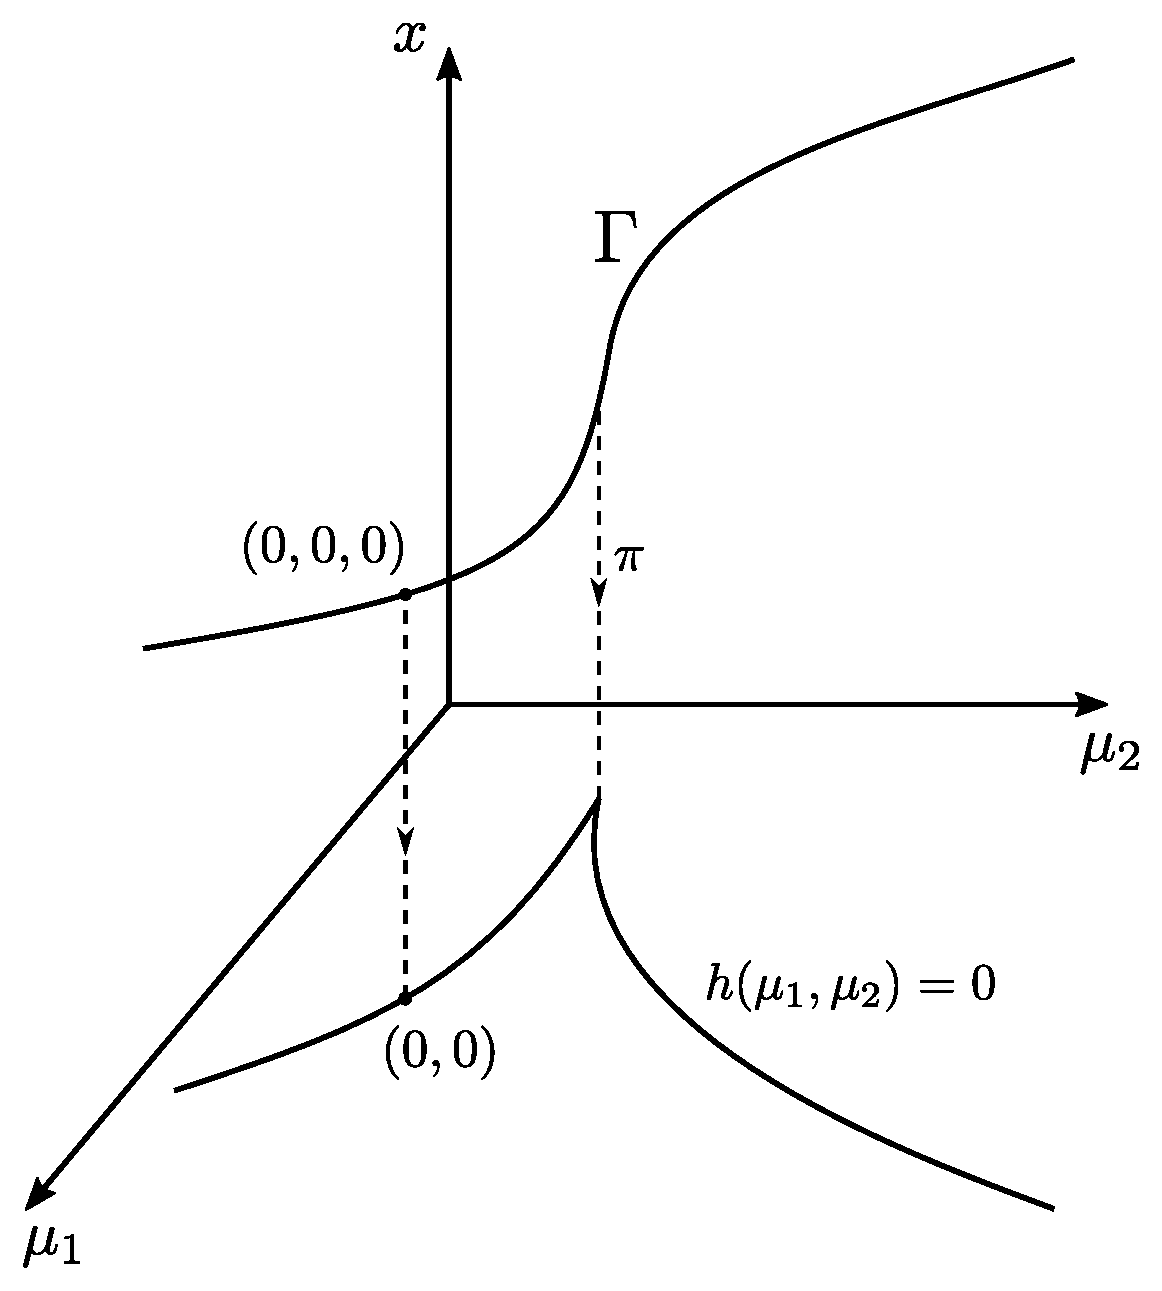
\includegraphics[width=0.50\linewidth]{figures/BifurcationCurveGamma.pdf}
    \end{center}
    \caption{A bifurcation curve $\Gamma$ and its corresponding bifurcation boundary $h(\mu_{1},\mu_{2})=0$ (projection onto the $(\mu_{1},\mu_{2})$-plane). Modified from Figure~8.1 in \citet{Kuznetsov2004}.}
    \label{fig:G2ModuleMass:BifurcationCurveGamma}
\end{figure}

If the extended system \eqref{equ:1DCase:ExtendedSystem} has a saddle-node bifurcation that is the carryover of the saddle-node bifurcation of interest in original system \eqref{equ:1DCase:OriginalSystem}, then this bifurcation must take place on $\Gamma$ as it is the set of points satisfying the conditions for a saddle-node bifurcation.

\begin{proposition}
    \label{the:1DCase:SaddleNodeBifurcationExtension1D}
    Consider the system \eqref{equ:1DCase:OriginalSystem}. Suppose $f(x;\mu_{1},\mu_{2})\in C^{2}(\mathbb{R}\times \mathbb{R}^{2},\mathbb{R})$ with a nonhyperbolic equilibrium at the origin, $f(0;0,0)=0$, $D_{x}f(0;0,0)=0$, and satisfying the nondegeneracy condition
    \begin{equation*}
        D_{xx}f(0;0,0)\neq 0,
    \end{equation*}
    and transversality condition for either $\mu_{1}$ or $\mu_{2}$
    \begin{equation*}
        D_{\mu_{1}}f(0;0,0)\neq 0 \quad \mathrm{or}\quad D_{\mu_{2}}f(0;0,0)\neq 0,
    \end{equation*}
    i.e., the system \eqref{equ:1DCase:OriginalSystem} has a saddle-node bifurcation where either $\mu_{1}$ or $\mu_{2}$ is the bifurcation parameter. This defines a one-dimensional smooth curve $\Gamma\subset \mathbb{R}^{3}$ in a neighbourhood of $(x,\mu_{1},\mu_{2})=(0,0,0)$ in which $f$ satisfies the singularity and nondegeneracy conditions.

    Consider the extended system \eqref{equ:1DCase:ExtendedSystem} by transforming parameter $\mu_{1}$ into a variable, where $f\in C^{2}(\mathbb{R}^{2}\times \mathbb{R},\mathbb{R})$ and $g\in C^{2}(\mathbb{R}\times\mathbb{R}, \mathbb{R})$. If there is a point $(x,\mu_{1},\mu_{2})=(x^{*},\mu_{1}^{*},\mu_{2}^{*})\in \Gamma$ such that $g(\mu_{1};\mu_{2})$ satisfies the singularity conditions
    \begin{equation}
        g(\mu_{1}^{*}; \mu_{2}^{*})=0, \quad D_{\mu_{1}}g(\mu_{1}^{*};\mu_{2}^{*})=b\neq 0,
        \label{equ:1DCase:Proposition1:SingularityConditions}
    \end{equation}
    and the transversality condition
    \begin{equation}
        \det\begin{pmatrix}
            D_{\mu_{1}}f & D_{\mu_{1}}g \\
            D_{\mu_{2}}f & D_{\mu_{2}}g
        \end{pmatrix} = D_{\mu_{1}}fD_{\mu_{2}}g - D_{\mu_{1}}gD_{\mu_{2}}f \neq 0,
      \label{equ:1DCase:Proposition1:TransversalityCondition}
    \end{equation}
    at $(x,\mu_{1},\mu_{2})=(x^{*},\mu_{1}^{*},\mu_{2}^{*})$, then the extended system  \eqref{equ:1DCase:ExtendedSystem} has a saddle-node bifurcation at $(x,\mu_{1})=(x^{*},\mu_{1}^{*})$ as $\mu_{2}$ crosses $\mu_{2}^{*}$.

    Moreover, there exists a unique function $\mu_{1}=\nu(\mu_{2})$ such that $\mu_{1}^{*}=\nu(\mu_{2}^{*})$, and the extended system is reduced to one dimension around $(x^{*},\mu_{1}^{*})$
    \begin{equation*}
        \dot \xi=f(\xi+\tfrac{a}{b}(\nu(\mu_{2})-\mu_{1}^{*})+x^{*}, \nu(\mu_{2});\mu_{2})-\tfrac{a}{b}g(\nu(\mu_{2});\mu_{2}),
    \end{equation*}
    where $\xi=x-x^{*}-\frac{a}{b}(\mu_{1}-\mu_{1}^{*})$ and $a=D_{\mu_{1}}f(x^{*},\mu_{1}^{*};\mu_{2}^{*})$.
\end{proposition}
\begin{proof}
    Let $z=(x, \mu_{1})^{T}$ and $F(z;\mu_{2})=F(x,\mu_{1};\mu_{2})=(f(x,\mu_{1};\mu_{2}),g(\mu_{1};\mu_{2}))^{T}$. By definition of $\Gamma$, the singularity conditions ($f=0$ and $D_{x}f=0$), the nondegeneracy condition ($D_{xx}f\neq0$), and one of the transversality conditions ($D_{\mu_{1}}f\neq0$ or $D_{\mu_{2}}f\neq0$) are satisfied at the point $(z^{*},\mu_{2}^{*})=(x^{*},\mu_{1}^{*},\mu_{2}^{*})\in\Gamma$. Since $g(\mu_{1}^{*};\mu_{2}^{*})=0$, we also have $F(x^{*},\mu_{1}^{*};\mu_{2}^{*})=0$ (first singularity condition for $F$). The Jacobian of $F$ evaluated at $z^{*}$ is
    \begin{equation*}
    A=D_{z}F(x^{*},\mu_{1}^{*};\mu_{2}^{*})=
    \left.\begin{pmatrix}
        D_{x}f & D_{\mu_{1}}f \\
        D_{x}g & D_{\mu_{1}}g
    \end{pmatrix}\right|_{z=z^{*}}=
    \begin{pmatrix}
        0 & a \\
        0 & b
    \end{pmatrix},
    \end{equation*}
    where $a=D_{\mu_{1}}f(x^{*},\mu_{1}^{*};\mu_{2}^{*})$ and $b=D_{\mu_{1}}g(\mu_{1}^{*};\mu_{2}^{*})\neq0$, by assumption \eqref{equ:1DCase:Proposition1:SingularityConditions}. Since $\det(A)=0$ and $\mathop\mathrm{tr}(A)=b\neq 0$, the eigenvalues of $A$ are $\lambda_{1}=0$ and $\lambda_{2}=b\neq 0$ with corresponding eigenvectors
    \[v_{\lambda_{1}}=\begin{pmatrix} 1 \\ 0 \end{pmatrix},
    \quad v_{\lambda_{2}}=\begin{pmatrix} a \\ b \end{pmatrix}.\]
    Note that condition $D_{\mu_{1}}g\neq0$ is needed to guarantee only one zero eigenvalue. Thus, $D_{z}F$ is singular with only one zero eigenvalue (second singularity condition for $F$).

    The diagonalization matrix $P$ and its inverse are given by
    \[P=\begin{pmatrix}
         1 & a \\
         0 & b
        \end{pmatrix}, \quad
    P^{-1}=\frac{1}{b}\begin{pmatrix}
         b & -a \\
         0 & 1
        \end{pmatrix}.
    \]
    Let the new shifted coordinates be defined by
    \begin{equation*}
        \begin{pmatrix}
            \xi \\
            \upsilon
        \end{pmatrix} = P^{-1}
        \begin{pmatrix}
            x-x^{*} \\
            \mu_{1} - \mu_{1}^{*}
        \end{pmatrix} =
        \begin{pmatrix}
            x -x^{*} - \frac{a}{b}(\mu_{1}-\mu_{1}^{*}) \\
            \frac{1}{b}(\mu_{1}-\mu_{1}^{*})
        \end{pmatrix}.
    \end{equation*}
    Then the corresponding extended system is given by
    \begin{equation*}
        \begin{aligned}
            \dot \xi &= f(\xi+a\upsilon+ x^{*}, b\upsilon + \mu_{1}^{*};\mu_{2}) - \tfrac{a}{b}g(b\upsilon + \mu_{1}^{*};\mu_{2}^{*}), \\
            \dot \upsilon & = \tfrac{1}{b}g(b\upsilon+\mu_{1}^{*};\mu_{2}^{*}).
        \end{aligned}
    \end{equation*}
    Define
    \begin{equation}
        f_{1}(\xi,\upsilon;\mu_{2})=f(\xi+a\upsilon+ x^{*}, b\upsilon + \mu_{1}^{*};\mu_{2}) - \tfrac{a}{b}g(b\upsilon + \mu_{1}^{*};\mu_{2}^{*}),
        \label{equ:1DCase:Proposition1:Proof:f1}
    \end{equation}
    and define $f_{2}(\upsilon; \mu_{2})$ such that
    \begin{equation*}
        \tfrac{1}{b}g(b\upsilon+\mu_{1}^{*};\mu_{2}^{*}) = b \upsilon + f_{2}(\upsilon;\mu_{2}).
    \end{equation*}
    Then,
    \begin{equation}
        \begin{aligned}
            \dot \xi &= f_{1}(\xi ,\upsilon;\mu_{2}), \\
            \dot \upsilon &= b \upsilon + f_{2}(\upsilon; \mu_{2}).
        \end{aligned}
        \label{equ:1DCase:Proposition1:Proof:Coordinates}
    \end{equation}

    Note that the singularity conditions are satisfied by construction,
    \begin{equation}
        \begin{aligned}
        & f_{1}(0,0;\mu_{2}^{*})=f_{2}(0;\mu_{2}^{*})=0, \\
%         & D_{\zeta}f_{1}(0,0;\mu_{2}^{*})=D_{\zeta}f_{2}(0,0;\mu_{2}^{*})=0, \\
        & D_{\xi}f_{1}(0,0;\mu_{2}^{*})=D_{\upsilon}f_{1}(0,0;\mu_{2}^{*})=D_{\xi}f_{2}(0;\mu_{2}^{*})=D_{\upsilon}f_{2}(0;\mu_{2}^{*})=0.
%         & D_{\xi}f_{1}(0,0;\mu_{2}^{*})=D_{x}f(x^{*},\mu_{1}^{*},\mu_{2}^{*})=0 \\
%         & D_{\nu}f_{1}(0,0;\mu_{2}^{*})=D_{x}f(x^{*},\mu_{1}^{*},\mu_{2}^{*}) a + D_{\mu_{1}}f(x^{*},\mu_{1}^{*},\mu_{2}^{*})b-\tfrac{a}{b}D_{\mu_{1}}gb=0
        \end{aligned}
        \label{equ:1DCase:Proposition1:Proof:NoLinearTerms}
    \end{equation}
    The nondegeneracy condition for $f_{1}$ is satisfied since
    \begin{equation*}
        D_{\xi\xi} f_{1}(0,0;\mu_{2}^{*}) = D_{xx}f(x^{*},\mu_{1}^{*};\mu_{2}^{*}))\neq0.
    \end{equation*}
    The transversality condition for $f_{1}$ follows from dividing the determinant in~\eqref{equ:1DCase:Proposition1:TransversalityCondition} by $-b\neq0$ and the definition of $f_{1}$ \eqref{equ:1DCase:Proposition1:Proof:f1}
    \begin{gather*}
        ( \cancelto{a}{D_{\mu_{1}}f(x^{*},\mu_{1}^{*};\mu_{2}^{*})} D_{\mu_{2}}g(\mu_{1}^{*};\mu_{2}^{*}) - \cancelto{b}{D_{\mu_{1}}g(\mu_{1}^{*};\mu_{2})} D_{\mu_{2}}f(x^{*},\mu_{1}^{*};\mu_{2}^{*}))\neq0,\\
        \implies D_{\mu_{2}}f(x^{*},\mu_{1}^{*};\mu_{2}^{*}) - \tfrac{a}{b}D_{\mu_{2}}g(\mu_{1}^{*};\mu_{2}^{*}) = D_{\mu_{2}}f_{1}(0,0;\mu_{2}^{*}) \neq 0.
    \end{gather*}
    Then, by Theorem~\ref{the:SaddleNodeBifurcationND} and Corollary~\ref{the:SaddleNodeBifurcationNDCorollary}, the transformed system \eqref{equ:1DCase:Proposition1:Proof:Coordinates} has a saddle-node bifurcation point at $(0,0)$ as $\mu_{2}$ crosses $\mu_{2}^{*}$.

    Transforming back to the variable $z$, we have that the extended system \eqref{equ:1DCase:ExtendedSystem} has a saddle-node bifurcation point at $(x^{*},\mu_{1}^{*})$ as $\mu_{2}$ crosses $\mu_{2}^{*}$.

    Now, denote
    \begin{equation*}
        F_{2}(\upsilon;\mu_{2})=b\upsilon +f_{2}(\upsilon;\mu_{2})=0.
    \end{equation*}
    Note that $D_{v}F_{2}(0;\mu_{2}^{*})=b\neq 0$, by equation \eqref{equ:1DCase:Proposition1:Proof:NoLinearTerms}. By the Implicit Function Theorem~\ref{the:ImplicitFunction}, there is a neighbourhood of $\mu_{2}=\mu_{2}^{*}$ where there exists a unique function $\upsilon=\hat\nu(\mu_{2})$ such that $\hat\nu(\mu_{2}^{*})=0$ and $F_{2}(\eta_{}(\mu_{2}),\mu_{2})=0$. Then, equation \eqref{equ:1DCase:Proposition1:Proof:Coordinates} reduces to
    \begin{equation*}
        \dot \xi = f_{1}(\xi ,\hat\nu(\mu_{2});\mu_{2}).
    \end{equation*}
    Changing back to $\mu_{1}$, we have
    \begin{gather*}
        \upsilon = \tfrac{1}{b}(\mu_{1}-\mu_{1}^{*}) \\
        \implies \mu_{1}=b\upsilon+\mu_{1}^{*}=b\hat\nu(\mu_{2})+\mu_{1}^{*}.
    \end{gather*}
    Define $\mu_{1}=\nu(\mu_{2}) = b\hat\nu(\mu_{2})+\mu_{1}^{*}$, then $\nu(\mu_{2}^{*})=b\hat\nu(\mu_{2}^{*})+\mu_{1}^{*}=\mu_{1}^{*}$.
    Finally, using the definition of $f_{1}(\xi,\nu,\mu_{2})$, we have
    \begin{align*}
        \dot \xi & = f_{1}(\xi ,\nu(\mu_{2});\mu_{2}) \\
        & = f_{1}(\xi,\tfrac{1}{b}(\nu(\mu_{2})-\mu_{1}^{*});\mu_{2}) \\
        & = f(\xi+\tfrac{a}{b}(\nu(\mu_{2})-\mu_{1}^{*})+x^{*}, \nu(\mu_{2});\mu_{2})-\tfrac{a}{b}g(\nu(\mu_{2});\mu_{2}) \\
        & = f(\xi+\tfrac{a}{b}(\nu(\mu_{2})-\mu_{1}^{*})+x^{*}, \nu(\mu_{2});\mu_{2})-\tfrac{a}{b}g(\nu(\mu_{2});\mu_{2}).
    \end{align*}
\end{proof}

This theorem provides a way to extend the scalar system \eqref{equ:1DCase:OriginalSystem} where a saddle-node occurs by transforming any parameter, $\mu_{1}$ for convenience, into a variable to obtain the extended system \eqref{equ:ExtendedSystem} where a saddle-node bifurcation now occurs as the other parameter, $\mu_{2}$, passes through some bifurcation value $\mu_{2}^{*}$. Note that the transformed parameter, $\mu_{1}$, does not need to be the original bifurcation parameter. Thus, we say that the saddle-node bifurcation in the extended system is the carryover of the saddle-node bifurcation in the original system. Also note that Proposition~\ref{the:1DCase:SaddleNodeBifurcationExtension1D} requires that $g(\mu_{1};\mu_{2})$ does not depend explicitly on $x$. This makes the conditions of this proposition easy to verify with graphical and numerical tools.

\begin{proposition}
    \label{the:1DCase:SaddleNodeBifurcationExtension1DCorollary}
    Under the conditions of Proposition~\eqref{the:1DCase:SaddleNodeBifurcationExtension1D}, let $h(\mu_{1},\mu_{2})=0$ be the projection of $\Gamma$ onto the $(\mu_{1},\mu_{2})$-plane. If $h(\mu_{1},\mu_{2})$ is differentiable at $(\mu_{1}^{*},\mu_{2}^{*})$, then conditions \eqref{equ:1DCase:Proposition1:TransversalityCondition} and \eqref{equ:1DCase:Proposition1:SingularityConditions} are equivalent to
    \begin{enumerate}
        \item $g(\mu_{1};\mu_{2})=0$ intersects $h(\mu_{1},\mu_{2})=0$ transversally at a point $(\mu_{1}^{*},\mu_{2}^{*})$, and
        \item the tangent line to $g(\mu_{1};\mu_{2})=0$ at $(\mu_{1}^{*},\mu_{2}^{*})$ is not parallel to the $\mu_{1}$-axis,
    \end{enumerate}
    respectively.
\end{proposition}


This proposition says that in order to find the saddle-node bifurcation points for the extended system, we plot the two-parameter bifurcation diagram of the smaller system, superimpose the nullclines of the new equation in the extended system, and look for transverse intersections between the saddle-node bifurcation curve and the nullclines. This is enough to verify the singularity and transversality conditions in the extended system.

\begin{proof}[Proof of Proposition~\ref{the:1DCase:SaddleNodeBifurcationExtension1DCorollary}]
    Note that $(\mu_{1}^{*},\mu_{2}^{*})$ satisfies $g=0$. Now, two vectors $u,v\in\mathbb{R}^{2}$ are transverse (parallel) if and only if the determinant of the matrix formed by them is non-zero (is zero), i.e.,
    \[det(u,v)=u_{1}v_{2}-v_{1}u_{2}=|u||v|\sin(\theta)\neq 0 \iff \theta \neq 0,\pi.\]

    Recall that $h(\mu_{1},\mu_{2})=0$ is defined by the projection of $\Gamma$ onto the $(\mu_{1},\mu_{2})$-plane, given by $(x,\mu_{1},\mu_{2},)\mapsto(\mu_{1},\mu_{2})$. Since at least one of $D_{\mu_{1}}f$ or $D_{\mu_{2}}f$ is non-zero, points on $\Gamma$ have a unique correspondence to points on $h(\mu_{1}, \mu_{2})=0$. Thus, a point $(\mu_{1}^{*},\mu_{2}^{*})$ at which $g=0$ and $h=0$ intersect has a unique corresponding point $(z^{*},\mu_{2}^{*})=(x^{*},\mu_{1}^{*}, \mu_{2}^{*})\in\Gamma$.

    Assume $D_{\mu_{1}}f\neq0$ at $(z^{*};\mu_{2}^{*})$. Then, by the Implicit Function Theorem~\ref{the:ImplicitFunction}, we can parameterize $\Gamma$ by $\mu_{2}$ with functions $x=\mathcal{X}(\mu_{2})$ and $\mu_{1}=\mathcal{M}(\mu_{2})$ such that $x^{*}=\mathcal{X}(\mu_{2}^{*})$ and $\mu_{1}^{*}=\mathcal{M}(\mu_{2}^{*})$ (see equation~\eqref{equ:1DCase:XandMfunctions}). Implicit differentiation of $f(x,\mu_{1};\mu_{2})=0$ with respect to $\mu_{2}$ gives
    \[D_{x}f\mathcal{X}'+D_{\mu_{1}}f\mathcal{M}'+D_{\mu_{2}}f=0.\]
    At $z^{*}$, $D_{x}f=0$ and we have
    \[\mathcal{M}'=-\frac{D_{\mu_{2}}f}{D_{\mu_{1}}f}.\]
    Implicit differentiation of $h(\mu_{1},\mu_{2})=0$ with respect to $\mu_{2}$ gives 
    \[D_{\mu_{1}}h\mathcal{M}'+D_{\mu_{2}}h=0.\]
    Evaluating at $z^{*}$, substituting the $\mathcal{M}'$ and multiplying by $-D_{\mu_{1}}f$, we obtain
    \begin{equation*}
        D_{\mu_{1}}hD_{\mu_{2}}f-D_{\mu_{2}}hD_{\mu_{1}}f=0.
    \end{equation*}
    This means that vectors $(D_{\mu_{1}}f,D_{\mu_{2}}f)^{T}$ and $(D_{\mu_{1}}h,D_{\mu_{2}}h)^{T}$ are multiple of each other at $z^{*}$. Note that this is also true if $D_{\mu_{1}}f=0$ since we must have $D_{\mu_{2}}f\neq0$ and similar arguments follow. Thus, $(D_{\mu_{1}}h,D_{\mu_{2}}h)^{T}$ and $(D_{\mu_{1}}g,D_{\mu_{2}}g)^{T}$ are transverse if and only if $(D_{\mu_{1}}f,D_{\mu_{2}}f)^{T}$ and $(D_{\mu_{1}}g,D_{\mu_{2}}g)^{T}$ are transverse, which is equivalent to saying that the transversality condition \eqref{equ:1DCase:Proposition1:TransversalityCondition} holds.

    Finally, the condition that the tangent line of $g(\mu_{1};\mu_{2})=0$ at $(\mu_{1}^{*},\mu_{2}^{*})$ is not parallel to the $\mu_{1}$-axis is clearly equivalent to $D_{\mu_{1}}g(\mu_{1}^{*},\mu_{2}^{*})\neq 0$.
\end{proof}

In the previous propositions, it is possible to generalize the arguments of the new scalar field, $g(\mu_{1};\mu_{2})$, to include dependence on $x$, i.e., $g(x,\mu_{1};\mu_{2})$, provided $\Gamma$ and $g=0$ intersect in the $(x,\mu_{1},\mu_{2})$-space. However, in the case of $g(\mu_{1};\mu_{2})$, the conditions of Proposition~\ref{the:1DCase:SaddleNodeBifurcationExtension1D} are easy to verify with graphical and numerical tools.

In order to illustrate the application of Propositions~\ref{the:1DCase:SaddleNodeBifurcationExtension1D} and \ref{the:1DCase:SaddleNodeBifurcationExtension1DCorollary}, we introduce the following examples, where we consider a one-dimensional system with two parameters, $a$ and $b$,
\[\dot x = f(x;a,b),\]
and transform the parameter $a$ into a variable to obtain the extended system
\[\left.\begin{aligned}
        \dot x &= f(x,a;b), \\
        \dot a &= g(a;b).
    \end{aligned}\right.\]

\begin{example}
    \label{exa:1DCase:Example1}
    Consider $f(x;a,b) = -a -b -x^2$. Since $D_{x}f=-2x=0$ at $x=0$, $D_{xx}f=-2\neq0$, and $D_{a}f=-1\neq0$, there is a saddle-node bifurcation at $x=0$ as $a$ crosses zero and $b=0$. Furthermore, since $D_{b}f=-1\neq0$, $b$ could be also taken as bifurcation parameter when $a=0$. The bifurcation boundary is given by $h(a,b)=-a-b=0$.  Figure~\ref{fig:1DCase:Example1}a shows the two-parameter bifurcation diagram along with the following three choices for $g(a;b)$.
    \begin{enumerate}
        \item If $g(a;b) = a+b$, then $g=0$ overlaps $h=0$ and they are never transverse. Indeed, the extended system does not have a saddle-node bifurcation since it always has a unique steady state at $(x,a)=(0,-b)$, for all values of $b$.
        \item If $g(a;b) = -a+b$, then $g=0$ intersects $h=0$ transversally at $(a,b)=(0,0)$. According to Proposition~\ref{the:1DCase:SaddleNodeBifurcationExtension1DCorollary}, the extended system has a saddle-node bifurcation at $(x,a)=(0,0)$ as $b$ crosses $b=0$. Indeed, there are two steady states, $(x,a)=(\pm\sqrt{-2b},b)$ when $b<0$, and they collide and disappear as $b$ becomes positive. Figure~\ref{fig:1DCase:Example1}b shows the bifurcation diagram for the extended system.
        \item If $g(a;b)=a^{2}-b$, then $g=0$ intersects $h=0$ transversally at $(a,b)=(0,0)$ and $(a,b)=(-1,1)$, but the tangent line of $g(a;b)=0$ at $(a,b)=(0,0)$ is parallel to the $a$-axis. Proposition~\ref{the:1DCase:SaddleNodeBifurcationExtension1DCorollary} guarantees the saddle-node bifurcation at $(x,a,b)=(0,-1,1)$, but not at $(x,a,b)=(0,0,0)$. In fact, at $(x,a,b)=(0,0,0)$, there is a Bogdanov-Takens (double-zero) bifurcation (see Section 8.4 in \citet{Kuznetsov2004}), since $D_{a}g=0$ implies that there are two zero eigenvalues. When $b=0$, there is a single steady state at $(x,a)=(0,0)$. When $0<b<1$, two steady states emerge from the origin, a stable node $(x,a)=(\sqrt{\sqrt{b}-b},-\sqrt{b})$, and saddle $(x,a)=(-\sqrt{\sqrt{b}-b},-\sqrt{b})$. When $b=1$ there is a saddle-node bifurcation at $(x,a)=(0,-1)$ as the two steady states collide and $D_{a}g\neq0$. Figure~\ref{fig:1DCase:Example1}c shows the bifurcation diagram for the extended system.
    \end{enumerate}
\end{example}

\begin{figure}
    \begin{center}
        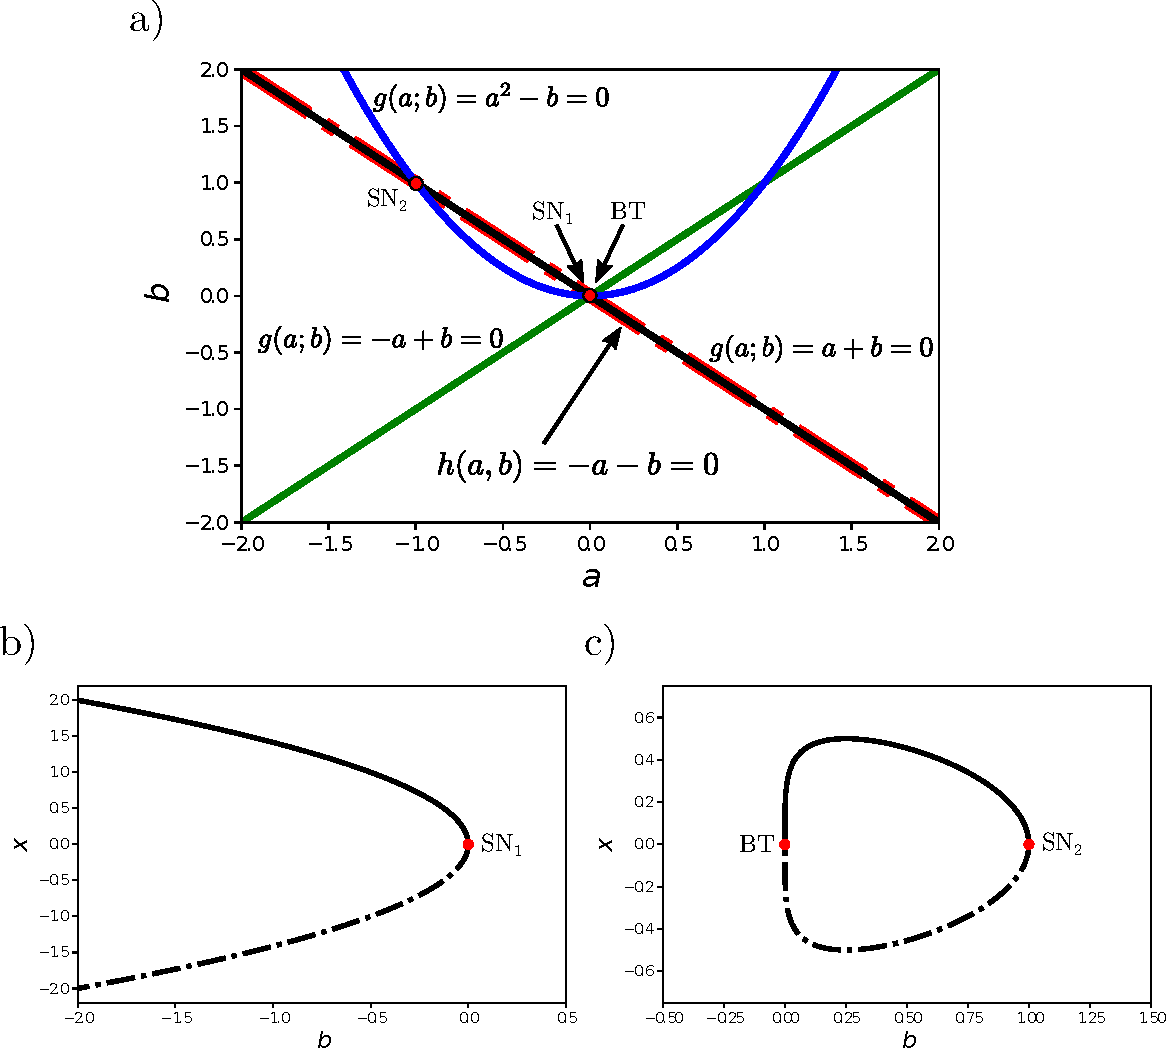
\includegraphics[width=\linewidth]{figures/Example1.pdf}
    \end{center}
    \caption[Bifurcation diagrams for Example \ref{exa:1DCase:Example1}.]{Bifurcation diagrams for Example \ref{exa:1DCase:Example1} where $f(x;a,b)=-a-b-x^2$. a) Two-parameter bifurcation boundary (red dash-dotted line) for $f$ with $a$ and $b$ as bifurcation parameters, and nullclines for three choices of $g(a;b)$: $g(a;b)=a+b$ (black) nullcline is never transverse; $g(a;b)=-a+b$ (green) nullcline is transverse at $(a,b)=(0,0)$; and $g(a;b)=a^{2}+b$ (blue) nullcline is transverse at $(a,b)=(-1,1)$ and $(a,b)=(0,0)$ but $D_{a}g(0;0)=0$. b) Bifurcation diagram when $g(a;b)=-a+b$. A saddle-node bifurcation (SN$_{1}$) occurs at $(x,a,b)=(0,0,0)$. c) Bifurcation diagram when $g(a;b)=a^{2}-b$. A saddle-node bifurcation (SN$_{2}$) occurs at $(x,a,b)=(0,1,1)$ and a Bogdanov-Takens (double-zero) bifurcation (BT) occurs at $(x,a,b)=(0,0,0)$.}
    \label{fig:1DCase:Example1}
\end{figure}


\begin{example}
    \label{exa:1DCase:Example2}
    Consider $f(x;a,b) = b^{2}+1 -a -x^2$. Since $D_{x}f=-2x=0$ at $x=0$, $D_{xx}f=-1\neq 0$, and $D_{a}f=-1\neq0$, there is a saddle-node bifurcation at $x=0$ as $a$ crosses $1$ and $b=0$. However, since $D_{b}f=2b=0$ at $b=0$, there is no saddle-node bifurcation at $(x,a,b)=(0,1,0)$ if $b$ is taken as bifurcation parameter. The bifurcation boundary is given by $h(a,b)=b^2+1-a=0$. Figure~\ref{fig:1DCase:Example2}a shows the two-parameter bifurcation diagram along with the following three choices for $g(b;a)$. Moreover, there is a saddle-node bifurcation at $x=0$ as $a$ crosses $b^{2}+1$, for fixed $b$.
    \begin{enumerate}
        \item If $g(a;b) = -a+2$, then $g=0$ intersects $h=0$ transversally twice, at $(a,b)=(2,\pm 1)$. Thus, by Proposition~\ref{the:1DCase:SaddleNodeBifurcationExtension1DCorollary}, the extended system undergoes two saddle-node bifurcations at $(x,a)=(0,2)$, one as $b$ crosses $b=-1$ from the left where the two steady states, $(x,a)=(\pm\sqrt{b^{2}-1},2)$, collide and disappear, and one as $b$ crosses $b=1$ from the left where the two steady states, $(x,a)=(\pm\sqrt{b^{2}-1},2)$, emerge. Figure~\ref{fig:1DCase:Example2}b shows the bifurcation diagram for the extended system.
        \item If $g(a;b) = -a+1$, then $g=0$ is tangential to $h=0$ at $(a,b)=(1,0)$. No saddle-node bifurcation occurs since the two steady states $(x,a)=(\pm\sqrt{b^{2}},1)=(\pm|b|,1)$ collide and bounce back, as seen in Figure~\ref{fig:1DCase:Example2}c. In fact, at $(x,a,b)=(0,1,0)$, the extended system satisfies the singularity conditions ($\lambda=0,-1$) and nondegeneracy condition ($D_{xx}f=-2\neq 0$), but not the transversality condition ($D_{a}fD_{b}g-D_{a}gD_{b}f=-2b|_{b=0}=0$). Note that this is not a transcritical bifurcation since the steady states $(|b|,1)$ and $(-|b|,1)$ are a stable node (two negative eigenvalues) and a saddle point (eigenvalues with opposite sign), respectively, for all $b$. In other words, they do not exchange stability when they collide, instead they touch and bounce back preserving their stability.
        \item If $g(a;b)=b-a+1$, then $g(a;b)=0$ is transverse at $(a,b)=(1,0)$ and $(a,b)=(2,1)$. Moreover, the tangent line to $g(a,b)=0$ at $(1,0)$ and $(2,1)$ is not parallel to the $a$-axis since $D_{a}g(a;b)=-1$. Thus, as in the first case ($g(a;b)=-a+2$), two saddle-node bifurcations occur, one as $b$ crosses $b=0$ from the left where two steady states $(x,a)=(\pm\sqrt{b(b-1)},b+1)$ collide and disappear, and one as $b$ crosses $b=1$ where two steady states $(x,a)=(\pm\sqrt{b(b-1)},b+1)$ emerge. Figure~\ref{fig:1DCase:Example2}d shows the bifurcation diagram for the extended system. This case is interesting because at $(a,b)=(1,0)$, the transversality condition is not satisfied for the original system with respect to $b$, i.e., $D_{b}f(0;1,0)=0$. In other words, even if $b$ is not a bifurcation parameter in the original system at $(x^{*},\mu^{*})$, $b$ becomes a bifurcation parameter in the extended system at the same point.
        \item If we extend the parameter $b$ instead using $\dot b= g(b;a)=b-a+1$, it follows from the previous case that two saddle-node bifurcations occur at $(x,a,b)=(0,1,0)$ and $(x,a,b)=(0,2,1)$, as seen in Figure~\ref{fig:1DCase:Example2}e. However, note that $b$ is not a bifurcation parameter in the original system at $(x,a,b)=(0,1,0)$ yet transforming $b$ into a variable there is a carryover of the saddle-node bifurcation that occurs in the original system with $a$ as bifurcation parameter.
    \end{enumerate}
\end{example}

\begin{figure}
    \begin{center}
        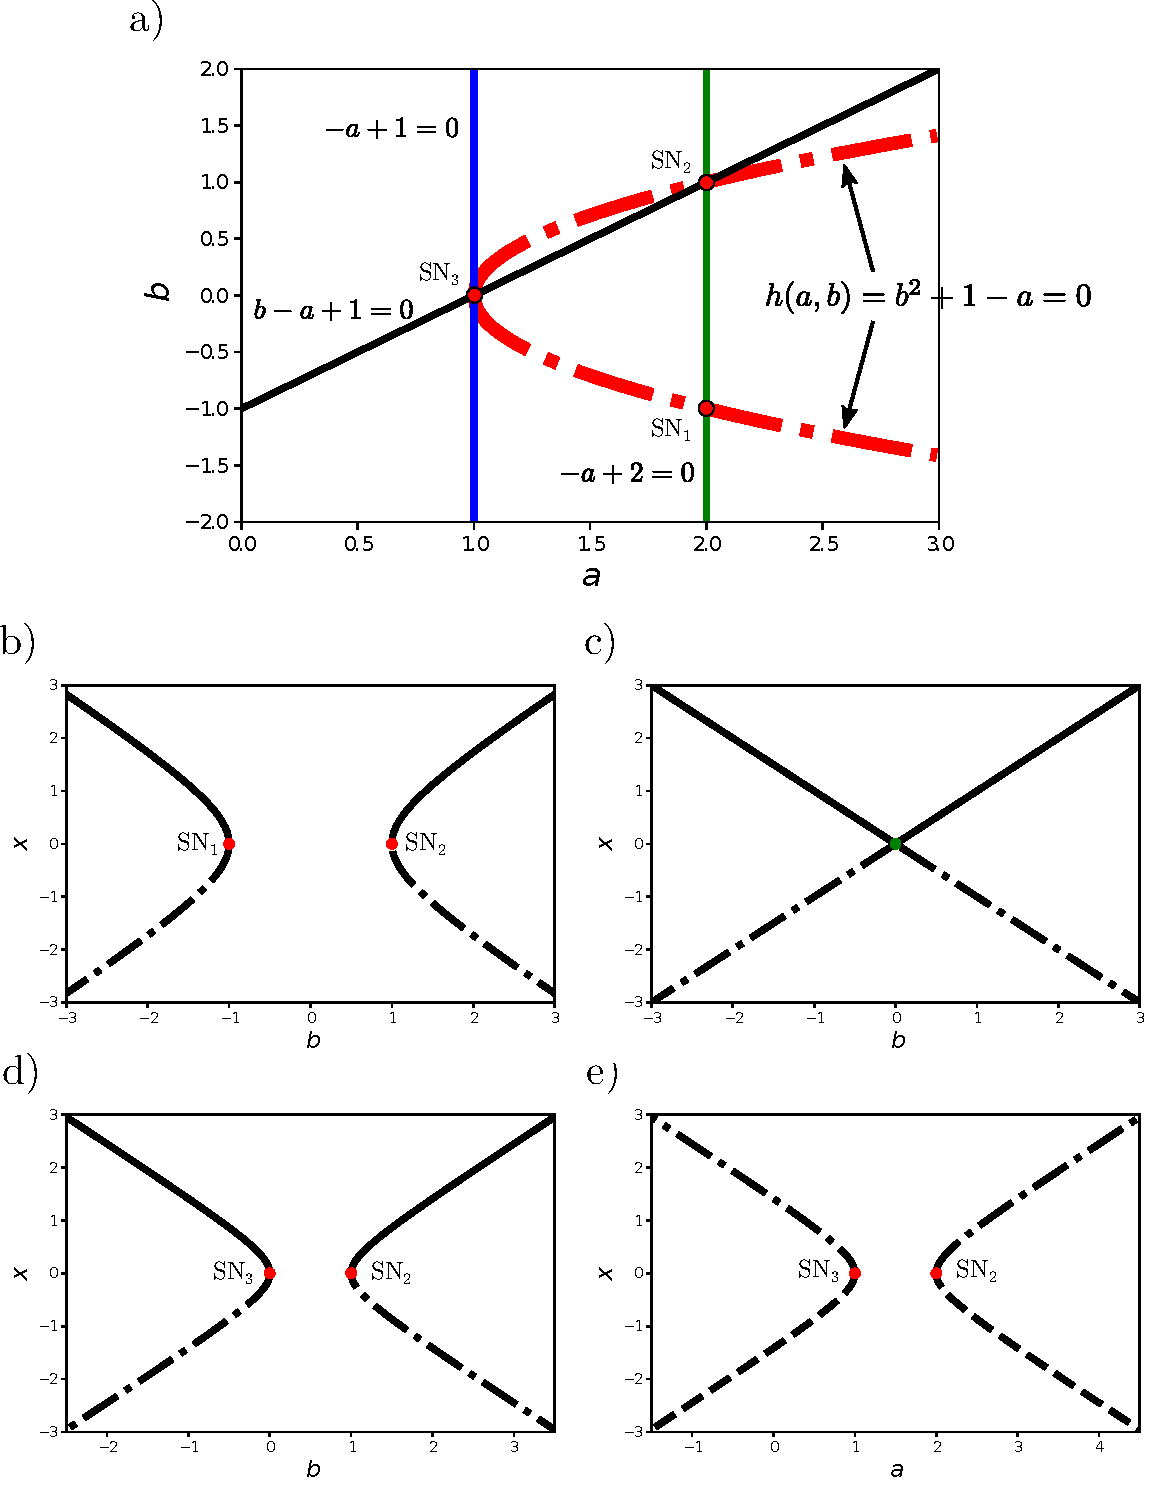
\includegraphics[width=0.95\linewidth]{figures/Example2.pdf}
    \end{center}
    \caption[Bifurcation diagrams for Example \ref{exa:1DCase:Example2}.]{Bifurcation diagrams for Example \ref{exa:1DCase:Example2} where $f(x;a,b)=b^{2}+1-a-x^2$. a) Two-parameter bifurcation boundary (red dash-dotted curve) for $f$ with $a$ and $b$ as \linebreak \null \hfill \emph{(continued})}
    \label{fig:1DCase:Example2}
\end{figure}
\begin{figure}
    %  \captionsetup{labelformat=contcaption,list=no}
     \ContinuedFloat
     \caption{bifurcation parameters, and nullclines for three choices of $g(a;b)$: $g(a;b)=-a+2$ (green) nullcline is transverse at $(a,b)=(2,-1)$ and $(a,b)=(2,1)$; $g(a;b)= -a+1$ (blue) is tangential at $(a,b)=(1,0)$; and $g(a;b)=b-a+1$ (black) nullcline is transverse at $(a,b)=(1,0)$ and $(a,b)=(2,1)$. b) Bifurcation diagram when $g(a;b)=-a+2$. Two saddle-node bifurcations occur at $(x,a,b)=(0,2,\pm1)$. c) Bifurcation diagram when $g(a;b)=-a+1$. No bifurcation occurs because the steady states collide but do not disappear. d) Bifurcation diagram when $g(a;b)=b-a+1$. Two saddle-node bifurcations occur at $(x,a,b)=(0,1,0)$ and $(x,a,b)=(0,1,1)$. e) Bifurcation diagram when $\dot b = g(a;b)=b-a+1$. Two saddle-node bifurcations occur at $(x,a,b)=(0,1,0)$ and $(x,a,b)=(0,2,1)$. }
\end{figure}


\section{$n$-dimensional case}
\label{sec:NDCase}


In the previous section, we showed the carryover of a saddle-node bifurcation in the one-dimensional case. In this section, we show that this result also holds in the $n$-dimensional case. In short, this is true because the saddle-node bifurcations can be reduced to one-dimension around the bifurcation point.

Suppose that $f$ in the original system \eqref{equ:OriginalSystem} satisfies the conditions of Theorem~\ref{the:SaddleNodeBifurcationND}. Then, we can reduce the system to one-dimensional form
\[\dot x = f_{1}(x,\eta(x;\mu_{1},\mu_{2});\mu_{1},\mu_{2}),\]
where functions $f_{1}(x,y;\mu_{1},\mu_{2})$ and $y=\eta(x;\mu_{1},\mu_{2})$ are given by the theorem, in a neighbourhood of $(x,y,\mu)=(0,0,0)$ in regards to the saddle-node bifurcation. Now, suppose that $f_{1}$ satisfies the transversality condition of Corollary~\ref{the:SaddleNodeBifurcationNDCorollary} for either $\mu_{1}$ or $\mu_{2}$. Then, in a similar fashion as in the one-dimensional case, the Implicit Function Theorem \ref{the:ImplicitFunction} guarantees the existence of an interval $I$ and unique functions $\mathcal{X}$ and $\mathcal{M}$ such $x$ and $\mu_{1}$ can be parameterized in terms of $\mu_{2}$ (for example), i.e.,
\begin{equation*}
    x=\mathcal{X}(\mu_{2}), \mu_{1}=\mathcal{M}(\mu_{2}), \mu_{2}\in I, \quad \mathrm{and}\quad  \mathcal{X}(0)=0, \mathcal{M}(0)=0.
\end{equation*}
This defines the smooth one-dimensional bifurcation curve
\begin{multline}
    \Gamma = \{ (z,\mu_{1},\mu_{2}) \colon 
    z = (x,y)=(\mathcal{X}(\mu_{2}),\eta(\mathcal{X}(\mu_{2});\mathcal{M}(\mu_{2}),\mu_{2})), \\ \mu_{1} = \mathcal{M}(\mu_{2}), \mu_{2}\in I \}.
%     \mathcal{X}(0)=0, \mathcal{M}(0)=0
%     \label{equ:NDCase:Gamma}
\end{multline}
To extend $\Gamma$ in this case, we take a point in $\Gamma$, different from $(x,y,\mu)=(0,0,0)$, and apply again Theorem~\ref{the:SaddleNodeBifurcationND} (after some appropriate translation) followed by the Implicit Function Theorem \ref{the:ImplicitFunction} as shown above. Note that functions $f_{1}$, $\mathcal{X}$, and $\mathcal{M}$ do not need to be the same as before. By continuity we can apply this process repetitive times and further extend $\Gamma$ as long as the transversality condition holds for either $\mu_{1}$ and $\mu_{2}$ at each step. Finally, the bifurcation boundary, $h(\mu_{1},\mu_{2})=0$, is defined by the projection of extended $\Gamma$ onto the $(\mu_{1},\mu_{2})$-plane, given by $\pi(z,\mu_{1},\mu_{2})\mapsto (\mu_{1},\mu_{2})$. Thus, the definition of $\Gamma$ and $h(\mu_{1},\mu_{2})=0$ is similar to the one-dimensional case.

\begin{proposition}
    \label{the:NDCase:SaddleNodeBifurcationExtensionND}
    Let $f(z;\mu_{1},\mu_{2})\in C^{2}(\mathbb{R}^{n}\times \mathbb{R}^{2},\mathbb{R}^{n})$ and suppose that the hypotheses of Theorem~\ref{the:SaddleNodeBifurcationND} are satisfied at $(z,\mu_{1},\mu_{2})=(0,0,0)$. Suppose also that the transversality condition in Corollary~\ref{the:SaddleNodeBifurcationNDCorollary} is satisfied for either $\mu_{1}$ or $\mu_{2}$. Let $m(\mu_{1},\mu_{2})$ be the extremal value defined in Theorem~\ref{the:SaddleNodeBifurcationND}. This defines a one-dimensional smooth curve $\Gamma\subset\mathbb{R}^{n+2}$ in a neighbourhood of $(z, \mu_{1}, \mu_{2})$ that satisfies the singularity and nondegeneracy conditions.

    Consider the extended system \eqref{equ:ExtendedSystem} by transforming parameter $\mu_{1}$ into a variable, where $f\in C^{2}(\mathbb{R}^{n+1}\times\mathbb{R},\mathbb{R}^{n})$ and $g\in C^{2}(\mathbb{R}\times\mathbb{R}, \mathbb{R})$. If there is a point $(z,\mu_{1},\mu_{2})=(z^{*},\mu_{1}^{*},\mu_{2}^{*})\in\Gamma$ such that $g(\mu_{1};\mu_{2})$ satisfies
    \begin{equation}
        g(\mu_{1}^{*};\mu_{2}^{*})=0, \quad b=D_{\mu_{1}}g(\mu_{1}^{*};\mu_{2}^{*})\neq 0,
        \label{equ:Proposition3:SingularityConditions}
    \end{equation}
    and the transversality condition
    \begin{equation}
        \det\begin{pmatrix}
            D_{\mu_{1}}m & D_{\mu_{1}}g \\
            D_{\mu_{2}}m & D_{\mu_{2}}g
        \end{pmatrix} = D_{\mu_{1}}hD_{\mu_{2}}g - D_{\mu_{1}}gD_{\mu_{2}}h \neq 0,
      \label{equ:Proposition3:TransversalityCondition}
    \end{equation}
    is satisfied at $(z,\mu_{1},\mu_{2})=(z^{*},\mu_{1}^{*},\mu_{2}^{*})$, then \eqref{equ:ExtendedSystem} has a saddle-node bifurcation at $(z,\mu_{1})=(z^{*},\mu_{1}^{*})$ as $\mu_{2}$ crosses $\mu_{2}^{*}$.
% TODO: Finish the extra part here. Finish also in the proof.
%     Moreover, there exists a unique function $\mu_{1}=\nu(\mu_{2})$ such that $\mu_{1}^{*}=\nu(\mu_{2}^{*})$, and the extended system is reduced to one dimension around $(x^{*},\mu_{1}^{*})$
%     \begin{equation*}
%         \dot \xi=f_{1}(\xi+\tfrac{a}{b}(\nu(\mu_{2})-\mu_{1}^{*})+x^{*}, \nu(\mu_{2});\mu_{2})-\tfrac{a}{b}g(\nu(\mu_{2});\mu_{2}),
%     \end{equation*}
%     where $\xi=x-x^{*}-\frac{a}{b}(\mu_{1}-\mu_{1}^{*})$, $a=D_{\mu_{1}}f_{1}(x^{*},\mu_{1}^{*};\mu_{2}^{*})$, and $f_{1}$ is given in Theorem~\ref{the:SaddleNodeBifurcationND}.
\end{proposition}
\begin{proof}
    First, we translate the point $z^{*}$ to the origin using a new variable $\zeta=z-z^{*}$ to obtain the translated system
    \begin{equation*}
        \dot \zeta = f(\zeta+z^{*};\mu_{1},\mu_{2}),
    \end{equation*}
    that satisfies all the conditions of Theorem~\ref{the:SaddleNodeBifurcationND} at $\zeta=0$.
    By Theorem~\ref{the:SaddleNodeBifurcationND}, we choose new translated coordinates $x\in\mathbb{R}$ and $y\in\mathbb{R}^{n-1}$ such that
    \begin{equation*}
        \begin{aligned}
            \dot x & = f_{1}(x,y;\mu_{1},\mu_{2}), \\
            \dot y & = My + f_{2}(x,y;\mu_{1},\mu_{2}),
        \end{aligned}
    \end{equation*}
    where $f_{1}=0$, $f_{2}=0$, $D_{x}f_{1}=0$, $D_{x}f_{2}=0$, $D_{y}f_{1}=0$, $D_{y}f_{2}=0$, and $D_{xx}f_{1}\neq0$ at $(x,y;\mu_{1},\mu_{2})=(0,0;\mu_{1}^{*},\mu_{2}^{*})$, and $M$ is invertible. Moreover, there is an interval $I(\mu_{1},\mu_{2})$ of 0 and function $y=\eta(x;\mu_{1},\mu_{2})$ where the extremal value 
    $$m(\mu_{1},\mu_{2})=\mathrm{Ext}_{x\in I(\mu_{1},\mu_{2})}[f_{1}(x,\eta(x;\mu_{1},\mu_{2});\mu_{1},\mu_{2})]$$
    is defined. Therefore, the system is reduced to one equation 
    $$\dot x=f_{3}(x;\mu_{1},\mu_{2})=f_{1}(x,\eta(x;\mu_{1},\mu_{2});\mu_{1},\mu_{2})$$ 
    in a neighborhood of $(\zeta,\mu_{1},\mu_{2})=(0,\mu_{1}^{*},\mu_{2}^{*})$ where the singularity and nondegeneracy conditions are satisfied. Then, the extended system \eqref{equ:ExtendedSystem} can be reduced to
    \begin{equation*}
        \begin{aligned}
            \dot x & = f_{3}(x,\mu_{1};\mu_{2})=f_{1}(x,\eta(x;\mu_{1},\mu_{2});\mu_{1},\mu_{2}), \\
            \dot \mu_{1} & = g(\mu_{1};\mu_{2}),
        \end{aligned}
    \end{equation*}
    in a neighborhood of $(\zeta,\mu_{1},\mu_{2})=(0,\mu_{1}^{*},\mu_{2}^{*})$. By assumption, the transversality condition, $D_{\mu_{i}}f_{1}\neq0$, is satisfied for either $\mu_{1}$ or $\mu_{2}$. Then, by Proposition~\ref{the:1DCase:SaddleNodeBifurcationExtension1D}, this system has a saddle-node bifurcation at $(x,\mu_{1})=(0,\mu_{1}^{*})$ as $\mu_{2}$ crosses $\mu_{2}^{*}$. It follows that the extended system \eqref{equ:ExtendedSystem} has a saddle-node bifurcation at $(z,\mu_{1})=(0,\mu_{1}^{*})$ as $\mu_{2}$ crosses $\mu_{2}^{*}$.
%TODO: Finish also in the proof. The existence of unique function $\mu_{1}=\nu(\mu_{2})$ follow similar arguments as in the proof of Proposition~\ref{the:1DCase:SaddleNodeBifurcationExtension1D}.
\end{proof}

As we might expect, Proposition~\ref{the:1DCase:SaddleNodeBifurcationExtension1DCorollary} also applies to the $n$-dimensional case. The proof follows similar arguments to the one-dimensional case.

\begin{proposition}
    \label{the:NDCase:SaddleNodeBifurcationExtensionNDCorollary}
    Under the conditions of Proposition~\eqref{the:NDCase:SaddleNodeBifurcationExtensionND}, let $h(\mu_{1},\mu_{2})=0$ be the projection of $\Gamma$ onto the $(\mu_{1},\mu_{2})$-plane. If $h(\mu_{1},\mu_{2})$ is diffe\-rentiable at $(\mu_{1}^{*},\mu_{2}^{*})$, then conditions \eqref{equ:Proposition3:TransversalityCondition} and  \eqref{equ:Proposition3:SingularityConditions} are equivalent to:
    \begin{enumerate}
        \item $g(\mu_{1};\hat\mu,\nu)=0$ intersects $h(\mu_{1},\mu_{2})=0$ transversally at a point $(\mu_{1}^{*},\mu_{2}^{*})$, and
        \item the tangent line to $g(\mu_{1};\mu_{2})=0$ at $(\mu_{1}^{*},\mu_{2}^{*})$ is not parallel to the $\mu_{1}$-axis,
    \end{enumerate}
    respectively.
\end{proposition}

\begin{example}
    \label{exa:NDCase:Example1}
    Consider the system
    \begin{equation*}
        \begin{aligned}
            \dot x &=\mu-x^{2}+xy-xy^{2},\\
            \dot y &=\lambda -y -x^{2}+x^{2}y,
        \end{aligned}
    \end{equation*}
    taken from \citet[p. 292]{Meiss2007}. There is a saddle-node bifurcation at the origin as $\mu$ crosses zero. The two-parameter bifurcation diagram starting from this bifurcation point is shown in Figure~\ref{fig:1DCase:Example3}a. Now, consider the extended system
    \begin{equation*}
        \begin{aligned}
            \dot x &=\mu-x^{2}+xy-xy^{2},\\
            \dot y &=\lambda -y -x^{2}+x^{2}y,\\
            \dot \mu &=g(\mu;\lambda) = \mu - \tfrac{1}{2}.
        \end{aligned}
    \end{equation*}
    The $\mu$-nullcline is transverse to the two-parameter bifurcation diagram in two points near $\lambda=0.5$ and $\lambda=1.1$ (see Figure~\ref{fig:1DCase:Example3}a). Since the tangent line of $g(\mu;\lambda)$ is not parallel to the $\mu$-axis at neither intersection, two saddle-node bifurcations are inherited with $\lambda$ as bifurcation parameter.
    Indeed, the bifurcation diagrams for $x$ and $y$ are shown in Figures~\ref{fig:1DCase:Example3}b and \ref{fig:1DCase:Example3}c, respectively. The corresponding bifurcation points are found to be
    \begin{equation*}
        \begin{aligned}
            (x,u,\mu;\lambda) \approx (-0.6792, 0.0604, 0.5; 0.4940),\\
            (x,u,\mu;\lambda) \approx (-0.8429, 1.2069, 0.5; 1.0599).
        \end{aligned}
    \end{equation*}
\end{example}


\begin{figure}
    \begin{center}
        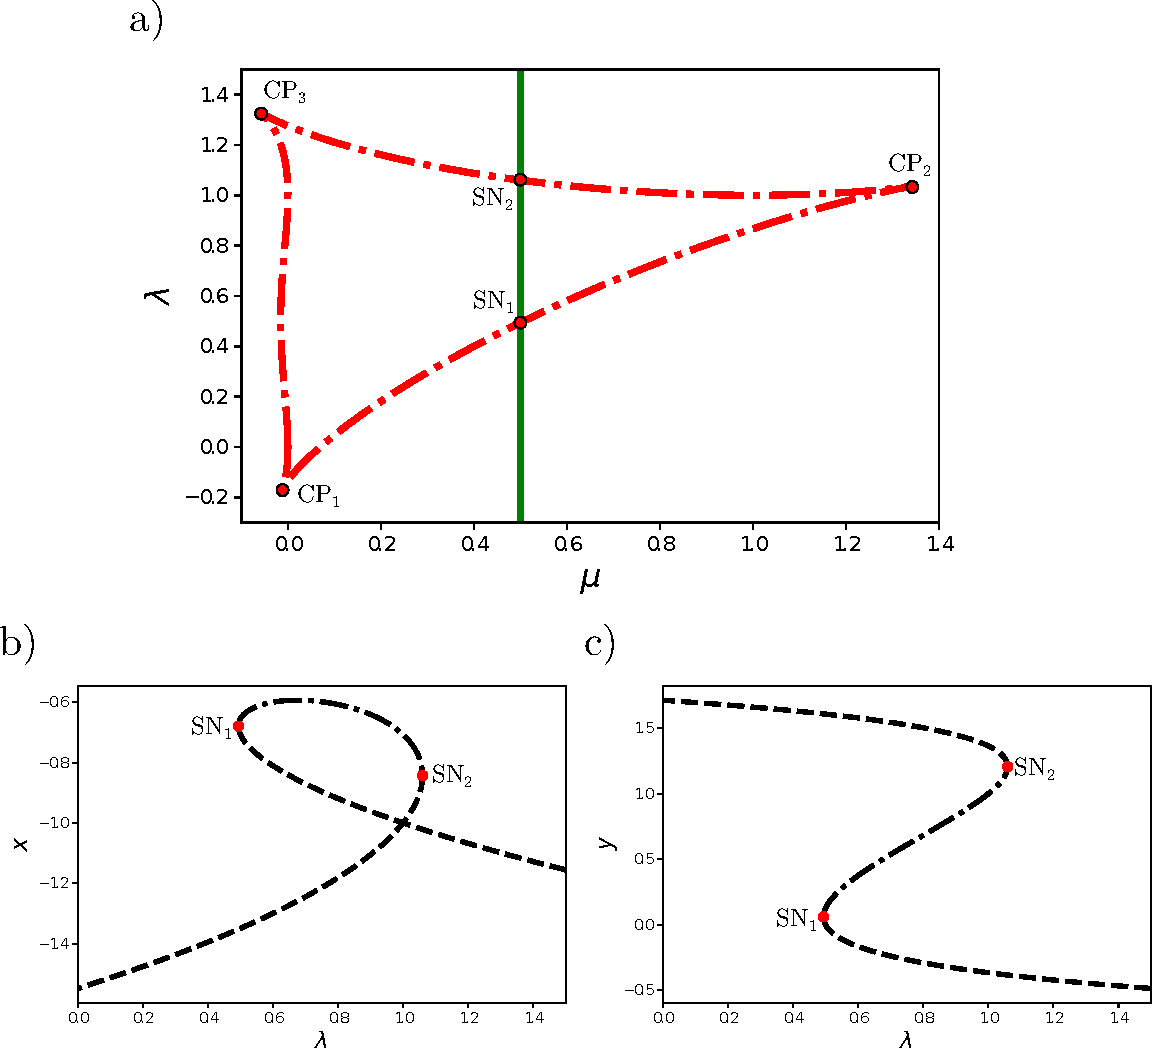
\includegraphics[width=\linewidth]{figures/Example3.pdf}
    \end{center}
    \caption[Bifurcation diagrams for Example \ref{exa:NDCase:Example1}.]{Bifurcation diagrams for Example \ref{exa:NDCase:Example1}. a) Two-parameter bifurcation boundary (red dashed-dotted curve) and nullcline for $g(\mu;\lambda)=\mu-\tfrac{1}{2}$ (green). Two saddle-node bifurcations (SN$_{1}$ and SN$_{2}$) occur at the transverse intersection between the $g$-nullcline and the bifurcation boundary. Note that there are cups bifurcations (CP$_{1}$, CP$_{2}$, and CP$_{3}$) associated with the system at the intersection of two saddle-node bifurcations. b-c) Bifurcation diagrams for the extended system with $\lambda$ as bifurcation parameter and variables $x$ and $y$ in the ordinate, respectively. The dashed lines indicate the unstable node with associated three-dimensional unstable manifold, while the dot-dashed lines indicate the saddle-node with associated one-dimensional stable manifold and two-dimensional unstable manifold.}
    \label{fig:1DCase:Example3}
\end{figure}


\section{Applications}

In this section we apply Propositions~\ref{the:NDCase:SaddleNodeBifurcationExtensionND} and \ref{the:NDCase:SaddleNodeBifurcationExtensionNDCorollary} to two models: the gen activation model \eqref{equ:Example:GenActivation:1D} and a model for the G2/M transition.


Consider the gen activation model \eqref{equ:Example:GenActivation:1D} where 
\[f(x;r,s)=s-rx+\frac{x^{2}}{1+x^{2}}.\]
This model is characterized by the existance of a saddle-node bifurcation as $s$ increases from zero when $r<\tfrac{1}{2}$. If the initial condition are $x(0)=0$, inceasing $s$ would drive a critical transition that brings the activity of gen $x$ to the high value equilibria, thus activating the gene. If the value of $s$ is decreased, the activity of the gen remains in the active mode (see Figure~\ref{fig:Example:GenActivation}).
The singularity conditions, $f=0$ and $D_{x}f=0$, give a parametrization of $r$ and $s$ in terms of $0< x\leq 1$
\[
r=\frac{2x}{(1+x^{2})^{2}}, \quad s = \frac{x^{2}(1-x^{2})}{(1+x^{2})^{2}},
\]
since $s\geq0$ and $r>0$. The nondegeneracy condition requires
\[
D_{xx}f = \frac{2(1-3x^{2})}{(1+x^{2})^{3}}\neq 0 \implies x\neq \frac{\sqrt{3}}{3},
\]
and the transversality conditions, $D_{s}f=1\neq$ and $D_{r}f=-x\neq 0 $, do not impose extra conditions. Thus, the bifurcation curve is given by
\begin{equation}
    \Gamma = \left\{ (x,r,s) : r=\frac{2x}{(1+x^{2})^{2}}, s = \frac{x^{2}(1-x^{2})}{(1+x^{2})^{2}}, x\in (0,1]\right\},
    \label{equ:Example:GenActivation:Gamma}
\end{equation}
and there is a saddle-node bifurcation at $(x,a,b)\in\Gamma$ such that $x\neq\frac{\sqrt{3}}{3}$. The two-parameter bifurcation curve on is shown in Figure~\ref{fig:Example:GenActivation}.


\begin{figure}
    \begin{center}
    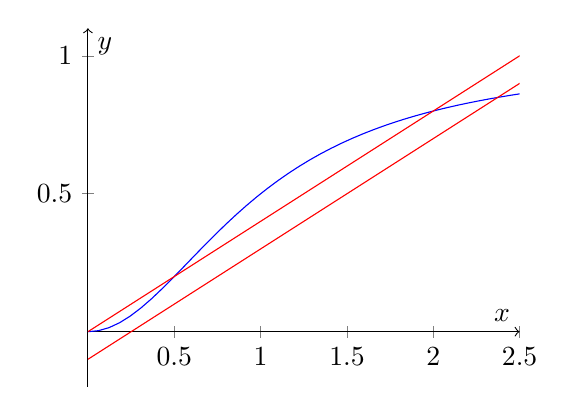
\begin{tikzpicture}
        \begin{axis}[
                xmin=0,xmax=2.5,
                ymin=-0.2,ymax=1.1,
                xlabel={$x$},
                ylabel={$y$},
                scale=0.8,
                ]
            \addplot [domain=0:3, samples=50, color=blue] ({x},{x^2/(1+x^2)});
            \addplot [domain=0:3, samples=50, color=red] ({x},{0.4*x});
            \addplot [domain=0:3, samples=50, color=red] ({x},{-0.1+0.4*x});
        \end{axis}
    \end{tikzpicture}
    \begin{tikzpicture}
        \begin{axis}[
                xmin=0,xmax=0.7,
                ymin=0,ymax=0.15,
                xlabel={$r$},
                ylabel={$s$},
                scale=0.8,
                ]
                \addplot [domain=0:1, samples=50] ({2*x/(1+x^2)^2},{x^2*(1-x^2)/(1+x^2)^2});
                \addplot [domain=0:1, samples=50,color=blue] ({0.4},{x});
                \addplot [domain=0:1, samples=50,color=red] ({0.6},{x});
        \end{axis}
    \end{tikzpicture}
    \end{center}
    \caption{Left: Phase plot. Right: Two-parameter bifurcation diagram.}
    \label{fig:Example:GenActivation}
\end{figure}

Now, consider transforming $r$ into a variable with linear synthesis and degradation terms
\begin{equation}
    \begin{aligned}
        \dot x & = f(x,r;s) = s - rx + \frac{x^{2}}{1+x^{2}}, \\
        \dot r & = g(r;s) = a - br.
    \end{aligned}
    \label{equ:Example:GenActivation:2D}
\end{equation}
where, $a>0$ and $b>0$.
According to Proposition \ref{the:1DCase:SaddleNodeBifurcationExtension1D}, there is a saddle-node bifurcation since the singularity conditions, $g=0$ and $D_{r}g=-b\neq 0$, and the transversality condition
\[\det\begin{pmatrix}
            D_{r}f & D_{r}g \\
            D_{s}f & D_{s}g
        \end{pmatrix} = 
        \begin{pmatrix}
            -x & -a\\
            1 & 0
        \end{pmatrix} = a \neq 0,\]
are satisfied for $(x,r,s)\in \Gamma$, with $r=c=\frac{a}{b}$. This is also shown in Figure~\ref{fig:Example:GenActivation} applying Proposition~\ref{the:1DCase:SaddleNodeBifurcationExtension1DCorollary} where the nullclines of $g=0$ corresponding to $c=0.4$ and $c=0.6$ cross the two-parameter bifurcation curve transversally. Moreover, if $c=0.4$, $x(0)=0$, and $s$ increases from zero crossing the bifurcation curve at $s\approx0.05$, the critical transition occurs and the gen is activated even after $s$ returns to zero. Since $r$ is dynamic, the exact value of $s$ for whic the gen is activated depends on the value of $r(0)$ but is close to $s\approx0.05$. 

[To do: type calculations and show there is a saddle-node bifurcation but using Theorem~\ref{the:SaddleNodeBifurcationND}.]

[To do: type G2 checkpoint and Cyclin activation application, or decide which of these two we should keep.]


\section{Discussion}
\label{sec:Discussion}

Given a system with a saddle-node bifurcation, we studied the manifestation of the saddle-node bifurcation when transforming one parameter into a variable. We call this property the carryover of a saddle-node bifurcation. We focused on the case where the new differential equation associated with the new variable does not depend on the rest of the variables. We showed that additional singularity and transversality conditions are sufficient for the carryover of the saddle-node bifurcation. We also find that such conditions can be verified graphically with a two-parameter bifurcation diagram.

In Section ~\ref{sec:1DCase}, we studied the scalar case, that is, the scalar system \eqref{equ:1DCase:OriginalSystem} has a saddle-node bifurcation at the origin as either $\mu_{1}$ or $\mu_{2}$ cross zero. Such a saddle-node bifurcation is characterized by singularity and non-degeneracy conditions, and a transversality condition for either $\mu_{1}$ and $\mu_{2}$ \citep{Meiss2007}. By the Implicit Function Theorem \ref{the:ImplicitFunction}, there exists a one-dimensional bifurcation curve $\Gamma\in\mathbb{R}^{3}$ in the neighborhood of zero where the singularity, non-degeneracy, and transversality conditions are satisfied \citep{Kuznetsov2004}. If we transform $\mu_{1}$ into a variable, we obtain the two-dimensional extended system \eqref{equ:1DCase:ExtendedSystem}. Any carryover of the saddle-node bifurcation to the extended system must take place in $\Gamma$. We proved that if 1) the $\mu_{1}$-nullcline intersects $\Gamma$ transversally, and 2) the new equation does not add another zero eigenvalue at the intersection, then the extended system has a saddle-node bifurcation at the intersection. These are the additional transversality and singularity conditions for the extended system, respectively (see Proposition~\ref{the:1DCase:SaddleNodeBifurcationExtension1D}).

Moreover, we showed that the transversality and singularity conditions for the extended system can be easily verified in the two-parameter bifurcation diagram with $\mu_{1}$ and $\mu_{2}$ as bifurcation parameters. The two-parameter bifurcation curve is the projection of $\Gamma$ onto the $\mu_{1}\mu_{2}$-plane. By superimposing the $\mu_{1}$-nullcline on the two-parameter, we can verify 1) the transversality condition if the $\mu_{1}$-nullcline intersects the two-parameter bifurcation curve transversally, and 2) the singularity condition if the $\mu_{1}$-nullcline is not parallel to the $\mu_{1}$-axis at the intersection (see Proposition~\ref{the:1DCase:SaddleNodeBifurcationExtension1DCorollary}). This graphical result is the consequence of the fact that the new equation does not depend on the other variable ($g(\mu_{1}; \mu_{2})$ does not depend on $x$). Thus, if the projection of $\Gamma$ and the $\mu_{1}$-nullcline intersect as seen from the $\mu_{1}\mu_{2}$-plane, then $\Gamma$ and the $\mu_{1}$-nullcline also intersect in $\mathbb{R}^{3}$.

Note that it is irrelevant which of the two parameters (or both) satisfies the transversality condition for the original system, we only need to start from a saddle-node bifurcation point and follow the bifurcation along $\Gamma$. In fact, $\Gamma$ can be extended as long as the transversality condition is satisfied for at least one of the parameters. Interestingly, a carryover can happen at a point where either $\mu_{1}$ (the transformed variable) or $\mu_{2}$ (the remaining parameter) is a bifurcation parameter in the original system. These cases were illustrated with examples in the text. It is still left to show that a carryover can happen at a point where the bifurcation happens as both $\mu_{1}$ and $\mu_{2}$ change simultaneously (but not individually), separately, or when $k$ parameters change simultaneously.

In Section ~\ref{sec:NDCase}, we extended our study to the $n$-dimensional case, that is, the $n$-dimensional system \eqref{equ:OriginalSystem} has a saddle-node bifurcation at the origin as either $\mu_{1}$ or $\mu_{2}$ cross zero and $\mu_{1}$ is transformed into a variable. We showed that the same singularity and transversality conditions apply in the carryover of the saddle-node bifurcation for the $n$-dimensional case. To show this, we reduced the original system in a neighborhood of the bifurcation point to one-dimension and applied our results for the scalar case. The $n$-dimensional case is also illustrated with an example.

The case where the new differential equation depends on the other variables, i.e., $\dot \mu_{1}=g(z,\mu_{1};\mu_{2})$, is not covered here. Assuming the bifurcation curve and the $\mu_{1}$-nullcline intersect in $\mathbb{R}^{n}$, an extra condition (or conditions) would be required to guarantee that the matrix $A$, as defined within the proof of Proposition \eqref{the:1DCase:SaddleNodeBifurcationExtension1D}, is invertible. We leave this case open for future research. We also leave open the interesting exploration of the carryover of other types of bifurcation (transcritical, pitchfork, Hopf, etc) as well as applications of the carryover of bifurcations.

The problem of the carryover of a saddle-node bifurcation was motivated by our results in Chapter~2, where we found an interesting, yet unclear, relationship between the SNIC$_{\text{Mass}}$ bifurcation and the SNIC$_{V_{c2}}$ bifurcation. In fact, studying Figure~(Figure in Chapter 2) motivated us to conjecture Proposition~\ref{the:NDCase:SaddleNodeBifurcationExtensionNDCorollary}, which indeed applies to conclude that the SNIC$_{V_{c2}}$ (locally, saddle-node) bifurcation is the carryover of the SNIC$_{\text{Mass}}$ (locally, saddle-node) bifurcation after transforming $Mass$ into a variable. Inaddition to clarifying the true origin of the SNIC$V_{c2}$ bifurcation, our results from this chapter are used in the next chapter.


% %% The Appendices part is started with the command \appendix;
% %% appendix sections are then done as normal sections
% %% \appendix
% 
% %% \section{}
% %% \label{}
% 
% %% References
% %%
% %% Following citation commands can be used in the body text:
% %% Usage of \cite is as follows:
% %%   \cite{key}          ==>>  [#]
% %%   \cite[chap. 2]{key} ==>>  [#, chap. 2]
% %%   \citet{key}         ==>>  Author [#]
% 
% %% References with bibTeX database:
% 
% % \bibliographystyle{model1-num-names}
% 
% %% New version of the num-names style
\bibliography{references}
% 
% %% Authors are advised to submit their bibtex database files. They are
% %% requested to list a bibtex style file in the manuscript if they do
% %% not want to use model1-num-names.bst.
% 
% %% References without bibTeX database:
% 
% % \begin{thebibliography}{00}
% 
% %% \bibitem must have the following form:
% %%   \bibitem{key}...
% %%
% 
% % \bibitem{}
% 
% \end{thebibliography}


\end{document}

